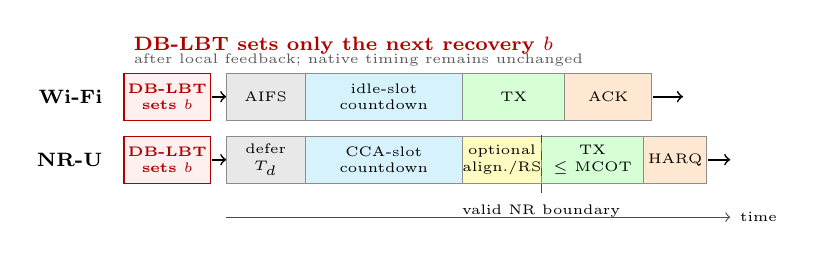
\begin{tikzpicture}[font=\scriptsize,x=1mm,y=1mm]
\tikzset{
  phase/.style={draw=black!45,minimum height=6mm,inner sep=0pt,
    align=center,text=black,font=\tiny},
  learned/.style={phase,draw=red!70!black,fill=red!6,
    text=red!70!black,font=\tiny\bfseries},
  native/.style={phase,fill=gray!18},
  countdown/.style={phase,fill=cyan!16},
  transmit/.style={phase,fill=green!16},
  feedback/.style={phase,fill=orange!18},
  alignment/.style={phase,fill=yellow!24}
}

\node[anchor=west,text=red!70!black,font=\scriptsize\bfseries]
  at (10,18.5) {DB-LBT sets only the next recovery $b$};
\node[anchor=west,text=black!65,font=\tiny]
  at (10,16.7) {after local feedback; native timing remains unchanged};

\node[anchor=east,font=\scriptsize\bfseries] at (8.5,12) {Wi-Fi};
\node[learned,minimum width=11mm] at (15.5,12) {DB-LBT\\sets $b$};
\draw[->,semithick] (21.2,12) -- (23,12);
\node[native,minimum width=10mm] at (28,12) {AIFS};
\node[countdown,minimum width=20mm] at (43,12) {idle-slot\\countdown};
\node[transmit,minimum width=13mm] at (59.5,12) {TX};
\node[feedback,minimum width=11mm] at (71.5,12) {ACK};
\draw[->,semithick] (77.2,12) -- (81,12);

\node[anchor=east,font=\scriptsize\bfseries] at (8.5,4) {NR-U};
\node[learned,minimum width=11mm] at (15.5,4) {DB-LBT\\sets $b$};
\draw[->,semithick] (21.2,4) -- (23,4);
\node[native,minimum width=10mm] at (28,4) {defer\\$T_d$};
\node[countdown,minimum width=20mm] at (43,4) {CCA-slot\\countdown};
\node[alignment,minimum width=10mm] at (58,4) {optional\\align./RS};
\node[transmit,minimum width=13mm] at (69.5,4) {TX\\$\leq$ MCOT};
\node[feedback,minimum width=8mm] at (80,4) {HARQ};
\draw[->,semithick] (84.2,4) -- (87,4);

\draw[dashed,black!70] (63,-0.2) -- (63,7.2);
\node[anchor=north,align=center,text=black,font=\tiny] at (63,-0.5)
  {valid NR boundary};
\draw[->,black!70] (23,-3.3) -- (87,-3.3)
  node[anchor=west,text=black,font=\tiny] {time};
\end{tikzpicture}
